%*****************************************
\chapter{Why night-time lights}\label{ch:whynighttimelights}
%*****************************************
%\setcounter{figure}{10}
% \NoCaseChange{Homo Sapiens}
Before proceeding with the data analysis, it is first necessary to dwell on the causal relationship between night-time lights and the economy. 
The first connection that needs to be made concerns the physical source of night-time lights which is simply light bulbs that run on electricity. Apart from naturally occurring night-time lights, it should be no surprise that electricity consumption (EC) is the primary cause of human light production observed from satellites (NTL).
\begin{figure}[h!]
    \centering
    \begin{tikzpicture}
        \node (x) at (0,0) [label=left:EC,point];
        \node (y) at (1.3,0) [label=right:NTL,point];
        \path (x) edge (y);
    \end{tikzpicture}
    \label{fig:my_label}
    \caption{Causal structure between electricity consumption and night-time lights.}
\end{figure}


Even if the direction of causation is unclear in the literature, GDP and electricity consumption are strictly connected, and the latter causes night-time lights.
\begin{figure}[h!]
    \centering
    \begin{tikzpicture}
        \node (z) at (1.3,1) [label=right:GDP,point];
        \node (x) at (0,0) [label=left:EC,point];
        \node (y) at (1.3,0) [label=right:NTL,point];
        \path (x) edge (y);
        \path[bidirected] (x) edge (z);
    \end{tikzpicture}
    \label{fig:my_label}
    \caption{Causal structure between GDP and night-time lights.}
\end{figure}

However, the connection between these two variables needs to be investigated more accurately. 
Electricity consumption enters fully into the production function of a country, i.e. it tells us the aggregate of how many industrial machines are currently running, how many electric motors are switched on, or how much air conditioning is used. While electricity consumption gives us an aggregate of the energy consumed in a country, night-time lights give us a particular portion of it. That is, that component of the consumed electricity that produces illumination. 
Moreover, the connection between the amount of light emitted and its distribution in space tells us a lot about the well-being of a country. 
Observing the lights emitted by North Korea, one is surprised by the very small amount of light emitted at night, so much so that South Korea looks like an island. Yet, assuming one can know the country's energy consumption, which is not disclosed, it is plausible that North Korea consumes far more energy than many other developing countries with more night-time lights. Although studies on this are few, it is likely that in North Korea, almost all of the available energy is used in war industries or propaganda activities, resulting in an extreme contraction of consumption due to home light rationing and brutal control of citizens' life.\footnote{\url{https://www.dailynk.com/english/north-koreas-electricity-situation-worsens-compared-to-last-year/}}\footnote{\url{https://www.cia.gov/the-world-factbook/countries/korea-north/}}
Therefore, even if military production fully enters into GDP, night-time lights allow us to study the actual energy used by the population and thus discriminate the economic well-being from the regime's propaganda parades and the enormous amount of energy that is forcibly subtracted from the population and conveyed to weapon production.
In other words, it is plausible to assume that night-time lights tell us more about the consumption component of the gross domestic product and of the population's living standards. Or, looking at the investment side, about the part that has a close connection with the population's consumption, namely: airports, theatres, highways or street lighting. 

Finally, as an obvious consequence, past literature has shown that night-time lighting is strongly affected by the consumption preferences of the living population of a country \citep{cinzano1999mapping}. 
In this sense, \cite{falchi2016new}, highlighted that Italy and South Korea are the most light-polluted countries in the world. This is undoubtedly due to their high living standards but also to country-specific characteristics such as consumption choices and spatial population distribution.

\section{Economic connections}
As previously stated, economic production is deeply involved with electricity consumption. From the elementary
national income identity in a closed economy:
\begin{equation}
    Y=C+I+G
\end{equation}
It is straightforward to see that each element on the right-hand side has a strict relation with night-time lights. For instance, after a growth in disposable income, individuals may decide to use the car more, maybe to reach an outdoor concert or visit a nearby city. These are all events that produce light consumption.
On the investment side, similar behaviour can be assumed. Due to increased taxation flows, governments may decide to build new infrastructures such as bridges, ports or railways, causing new massive light production. 
For these reasons, night-time lights can be used as a proxy for GDP.
\subsection{Roads}
Roads and highways provide valuable information on investment and consumption within a country. The set of new infrastructure is part of the investment component, which is an important determinant of GDP. The same can be sustained with the upgrade to new lighting technology dismissing the old one, as in the case of led street lamps.
At the same time, road traffic tells us a lot about the movement of people and thus the consumption component. Queues and traffic tell an eloquent story about the dynamism of a country and the number of people moving at a certain time.


\begin{figure}[h!]
    \hspace*{-2.8cm}
    \centering
    \subfloat[\centering Google Maps]{{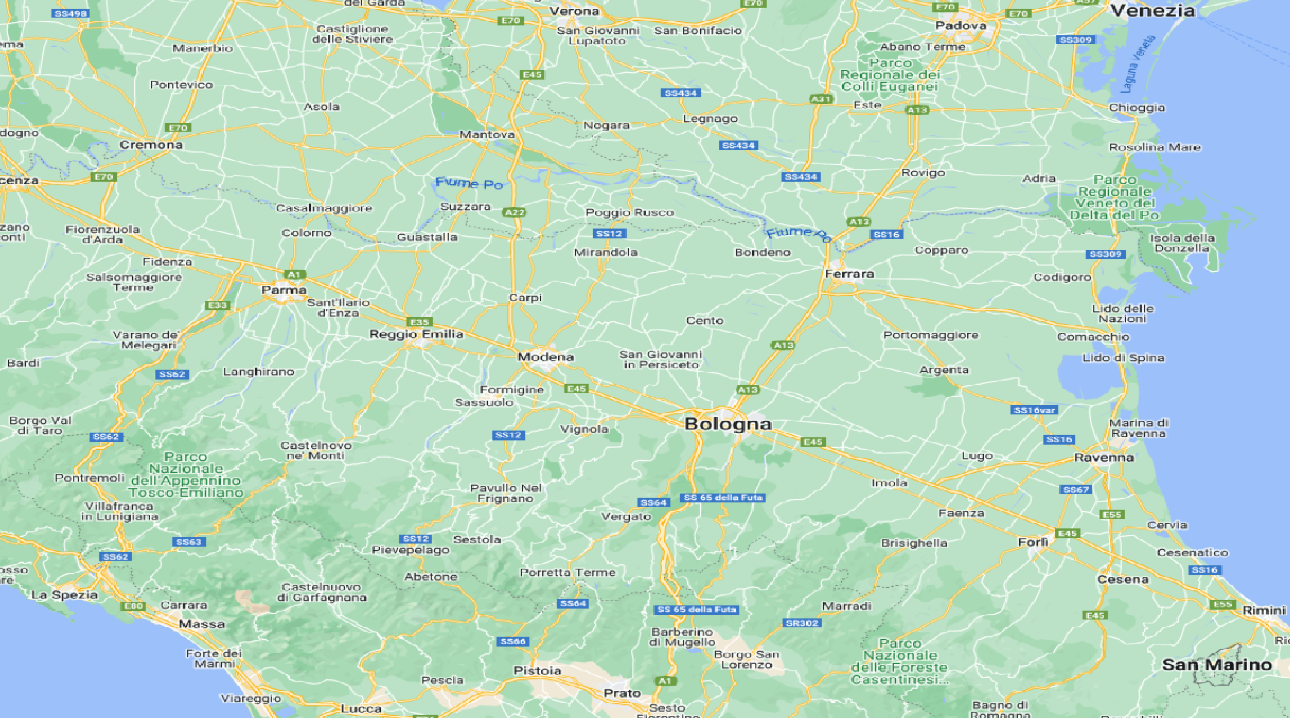
\includegraphics[width=8cm]{images/northitaroads_maps.png} }}%
    \subfloat[\centering Night-time lights]{{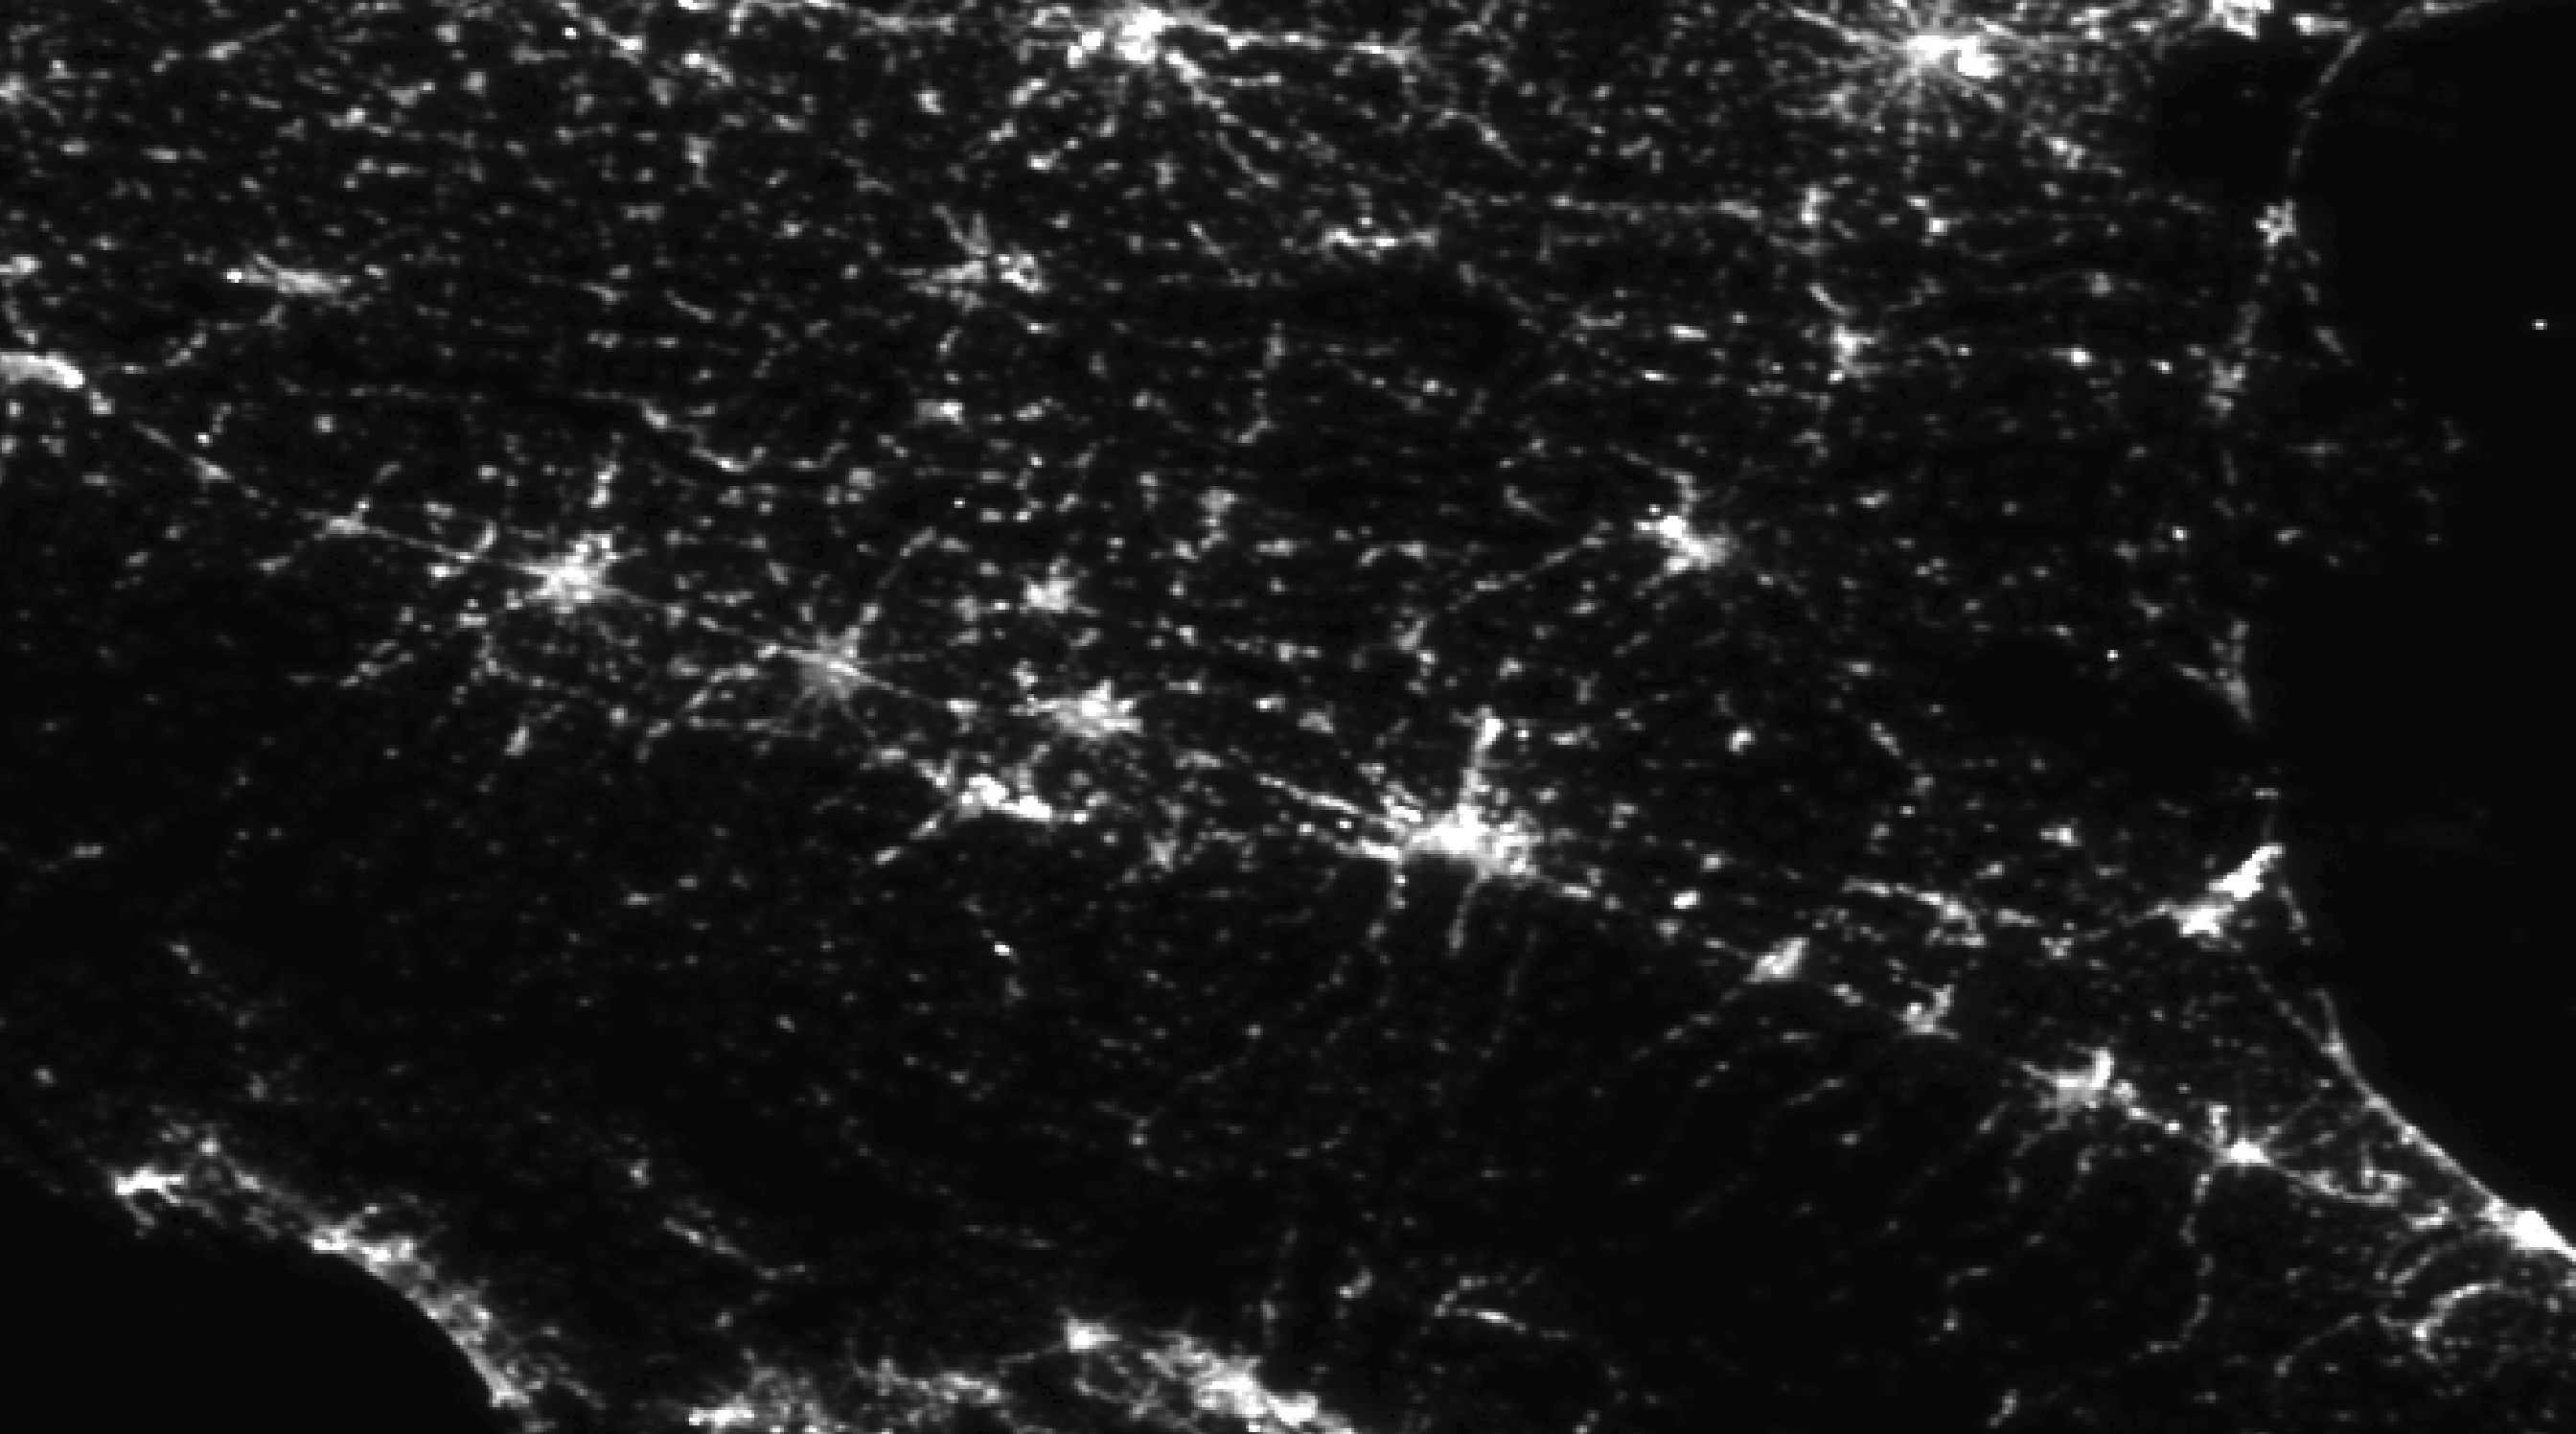
\includegraphics[width=8cm]{images/northitaroads_night.png} }}%
    \caption{North Italy roads - A1 and A14 highways connecting Bologna and Modena with Milan.}%
    \label{fig:northitalyroads}
\end{figure}

\begin{figure}
    \hspace*{-2.8cm}
    \centering
    \subfloat[\centering Google Maps]{{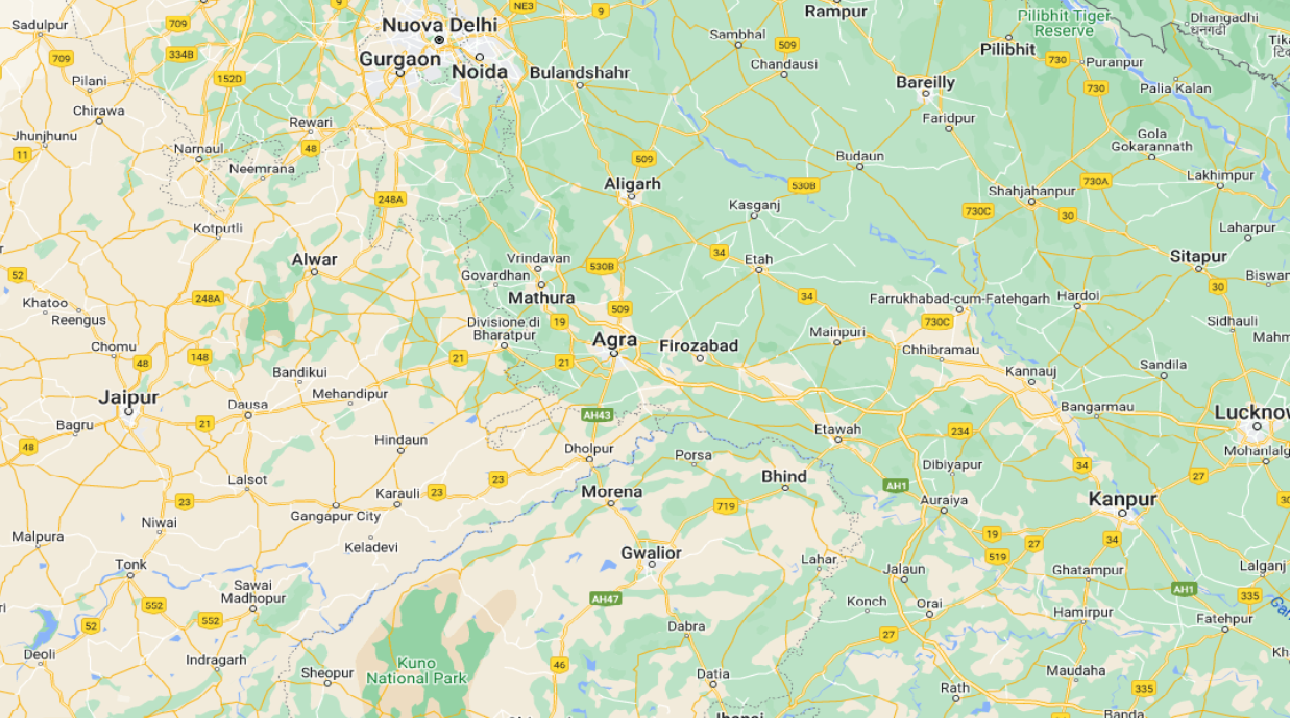
\includegraphics[width=8cm]{images/delhiroads_maps.png} }}%
    \subfloat[\centering Night-time lights]{{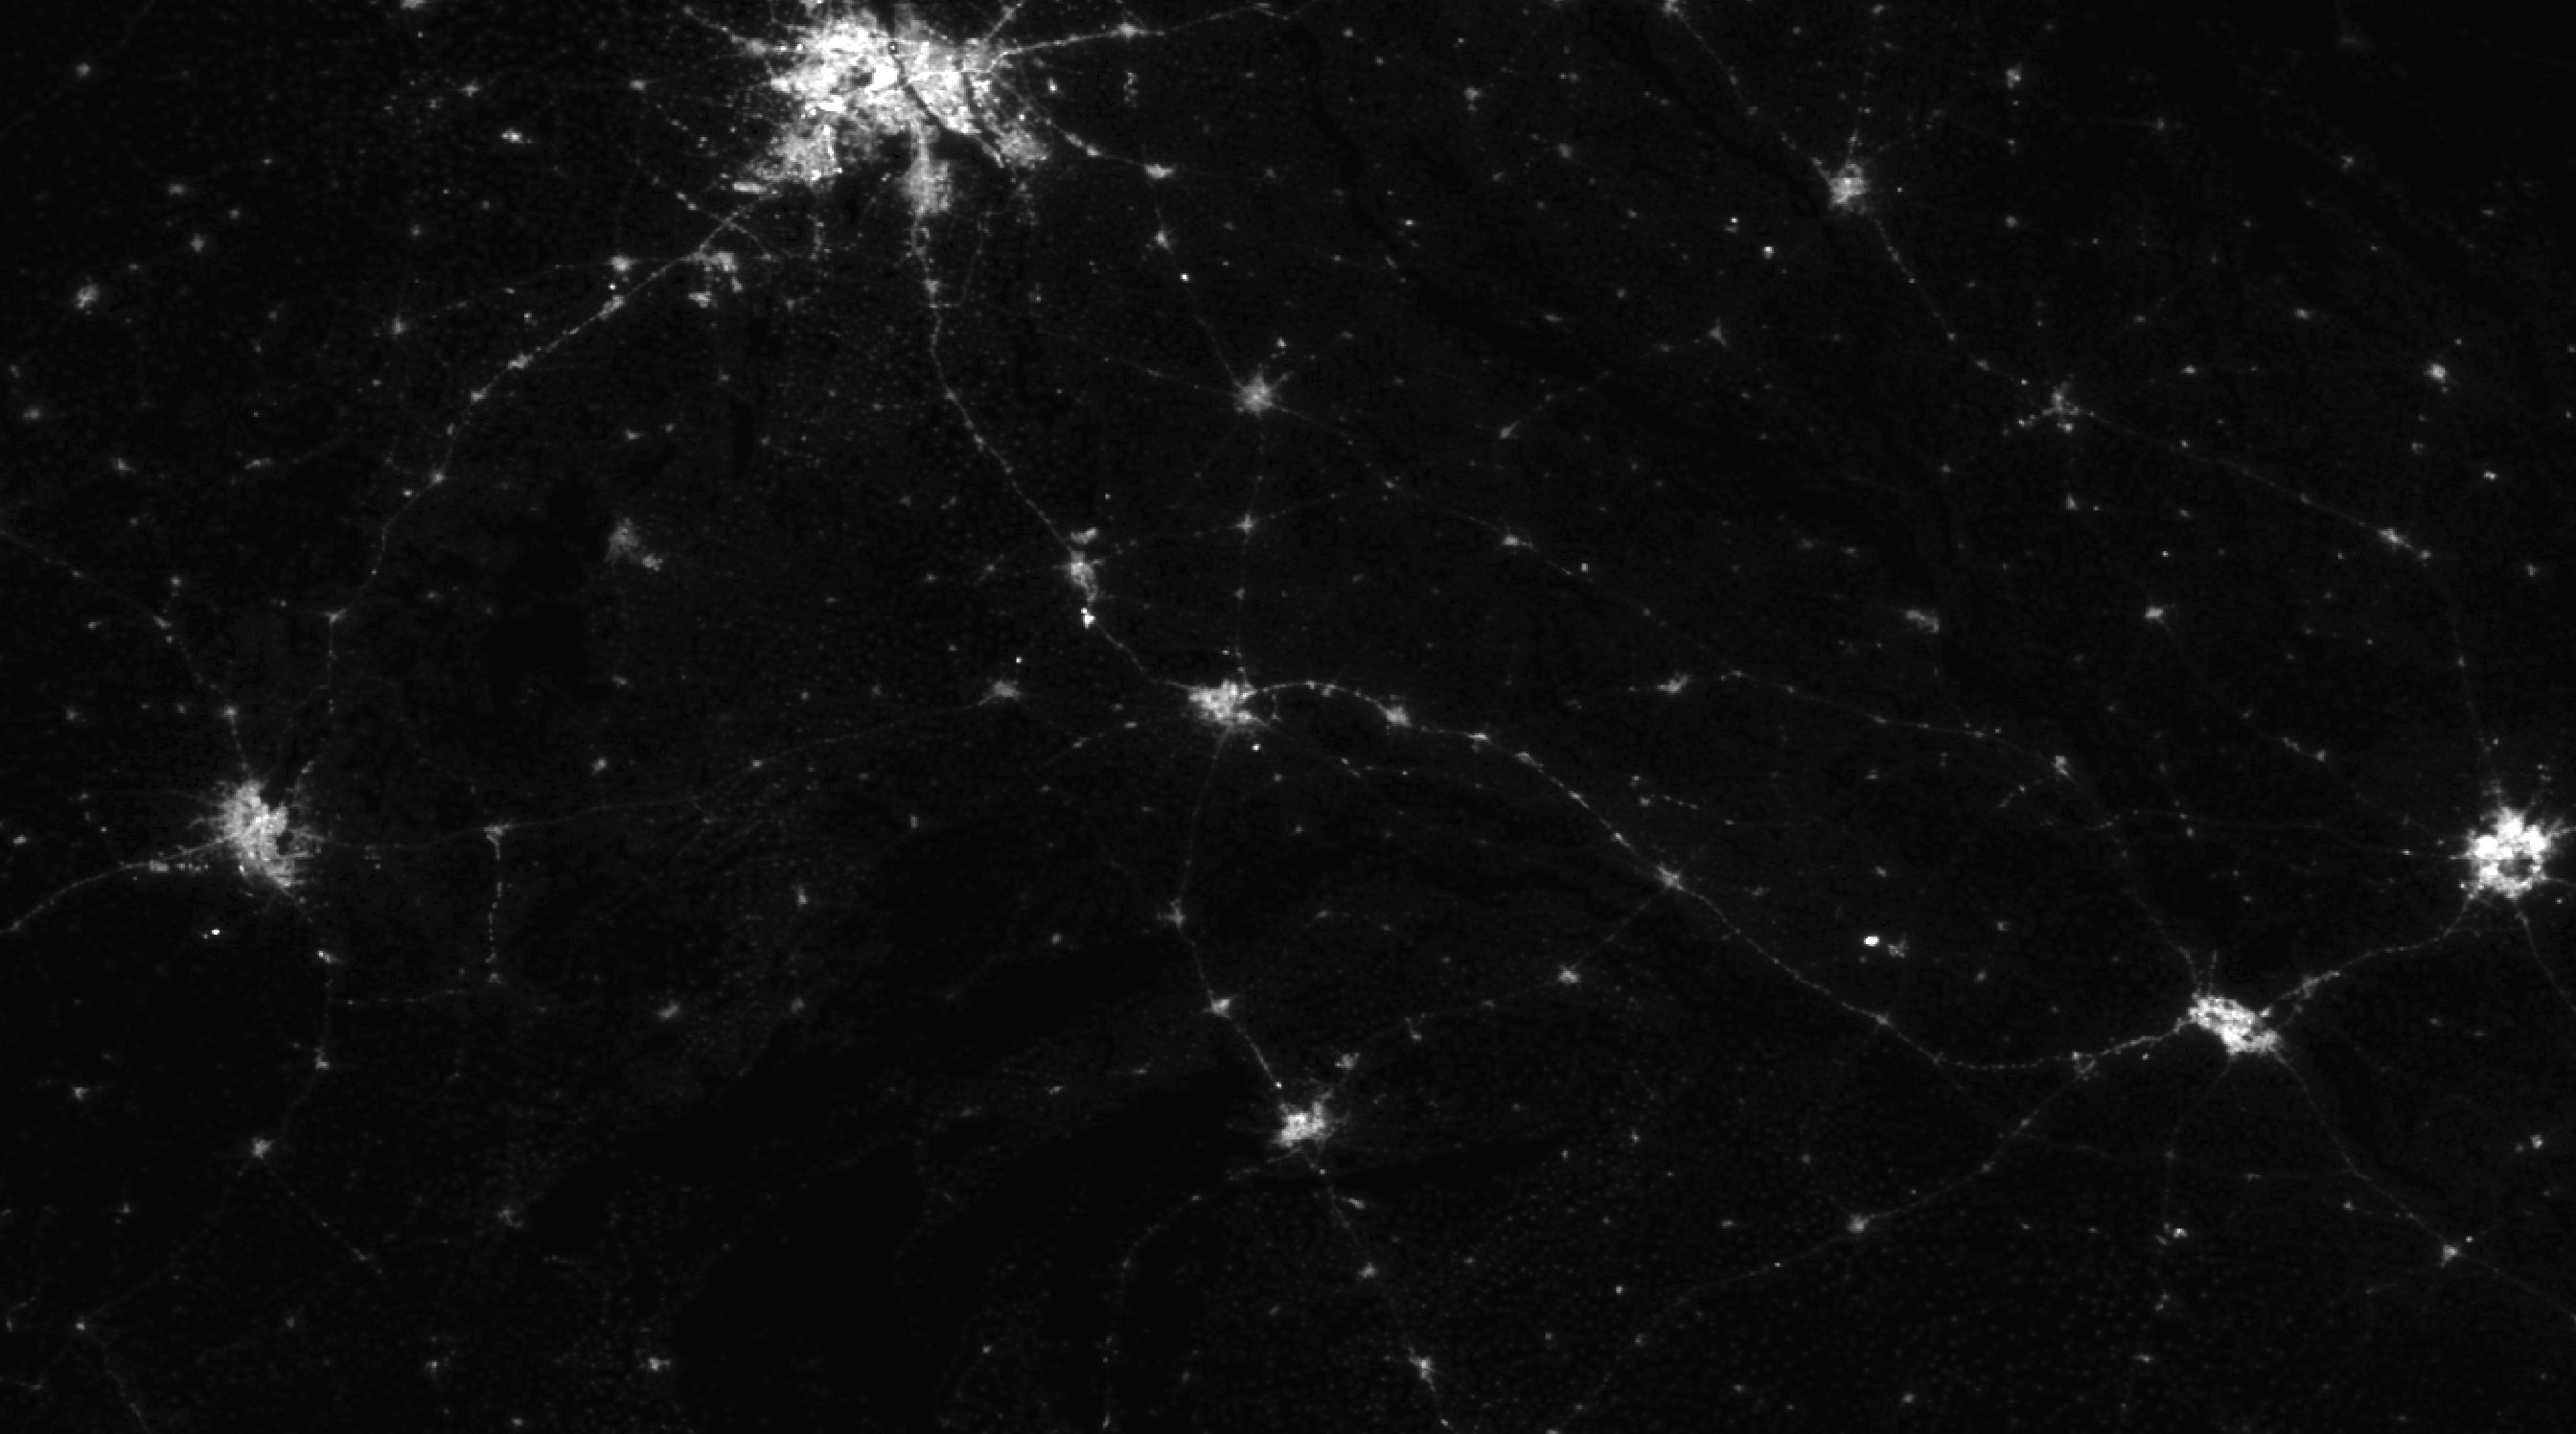
\includegraphics[width=8cm]{images/delhiroads_night.png} }}%
    \caption{New Delhi periphery roads.}%
    \label{fig:newdelhiroads}
\end{figure}
Observing night-time lights, the lines of communication between cities or towns can be studied in depth. \autoref{fig:northitalyroads} shows an extract of the main communication line in northern Italy, namely the A1 and A14 motorways connecting the cities of Bologna and Modena with Milan, some of the country's most productive areas. \autoref{fig:newdelhiroads}, on the other hand, shows an excerpt of the roads connecting New Delhi in India and peripheral cities.

\subsection{Cities}
Cities are the primary producers of night-time lights. Studying satellite imagery, the geographical distribution of urban settlements and some of the brightest elements of the cities can be observed, such as major roads,  airports and ports.
Cities' night-time lights can be a proxy for many economic-related variables. That is population concentration, city dynamism and traffic. It can also be assumed that brighter cities are more economically active and have the resources to maintain such electrical consumption.
\begin{figure}[h!]
    \hspace*{-2.8cm}
    \centering
    \subfloat[\centering Google Maps]{{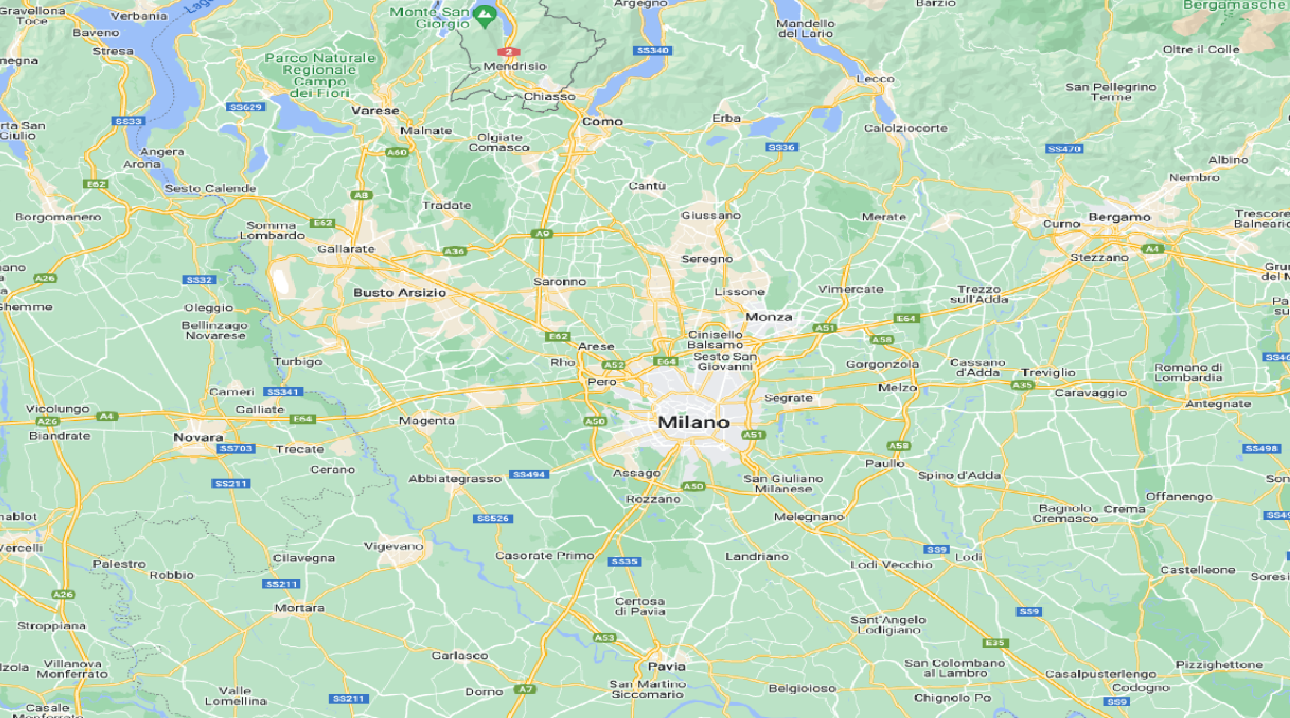
\includegraphics[width=8cm]{images/milan_maps.png} }}%
    \subfloat[\centering Night-time lights]{{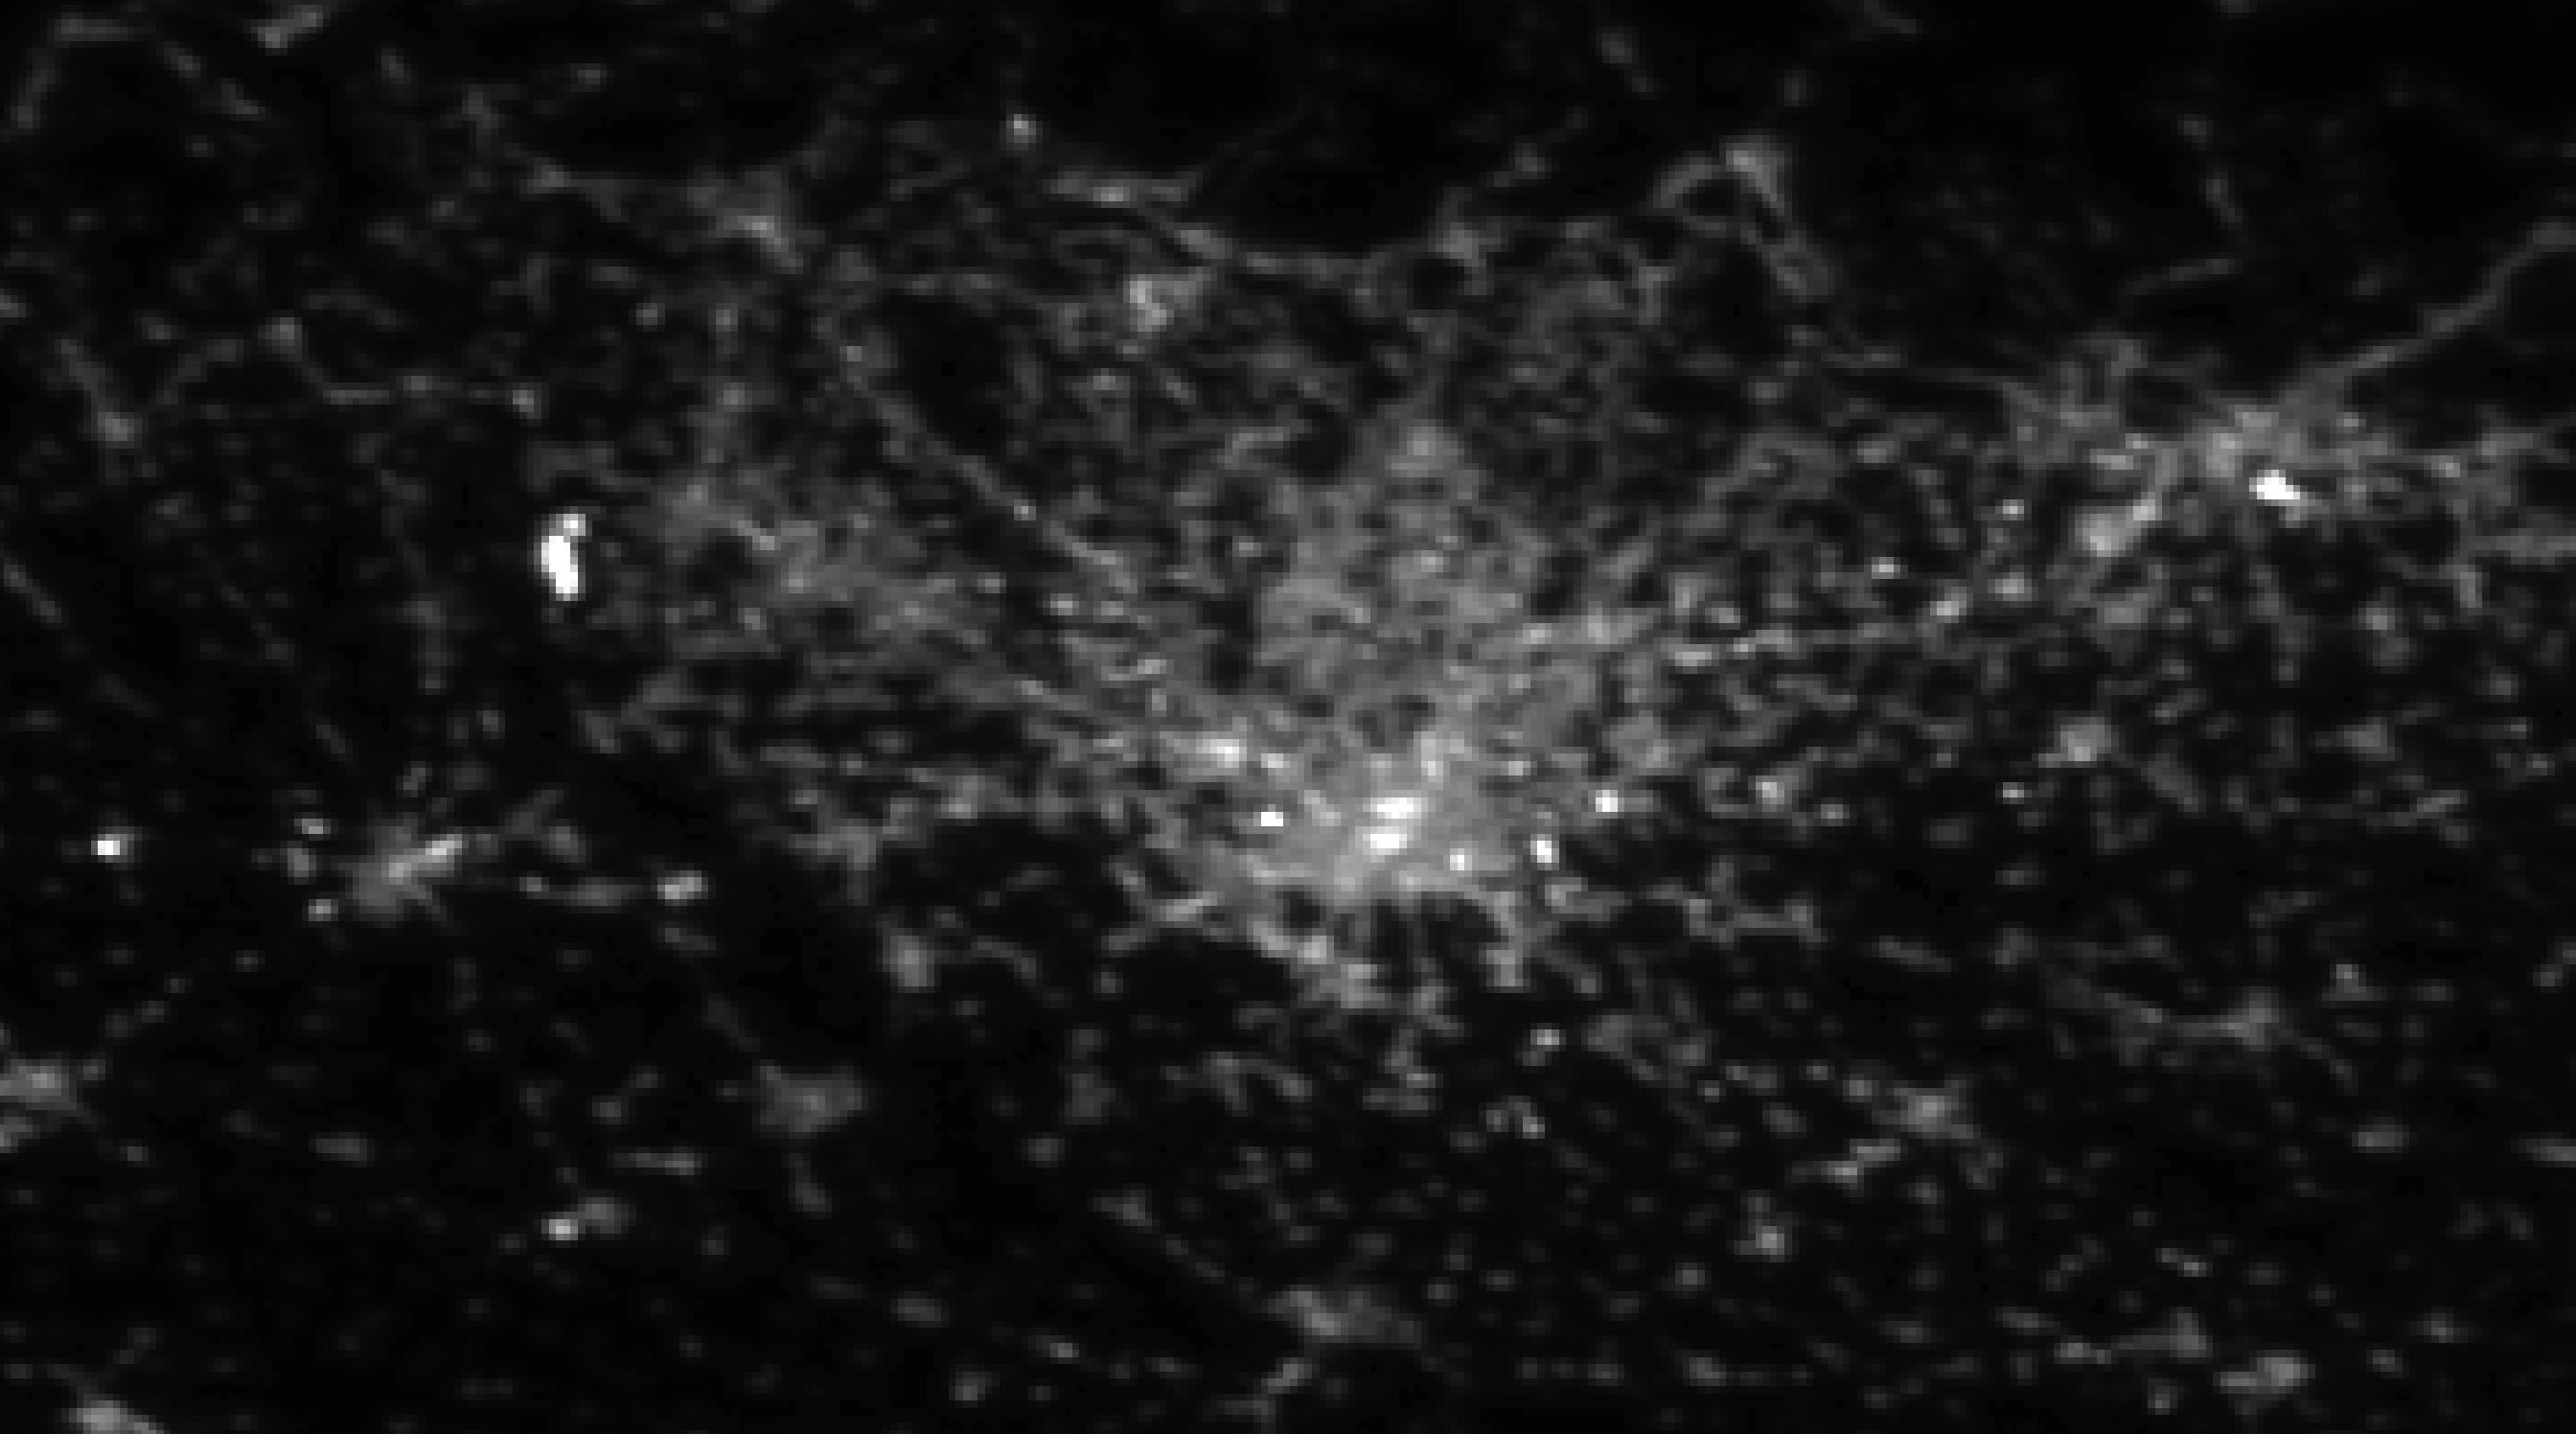
\includegraphics[width=8cm]{images/milan_night.png} }}%
    \caption{Milan - Italy.}%
    \label{fig:milan}
\end{figure}

\autoref{fig:milan} shows the city of Milan and \autoref{fig:london} shows London. They are both characterized by well-known web shapes. It can be recognized some roads connecting points of interest of the cities and the main airports of both cities can be easily individuated.
\begin{figure}[h!]
    \hspace*{-2.8cm}
    \centering
    \subfloat[\centering Google Maps]{{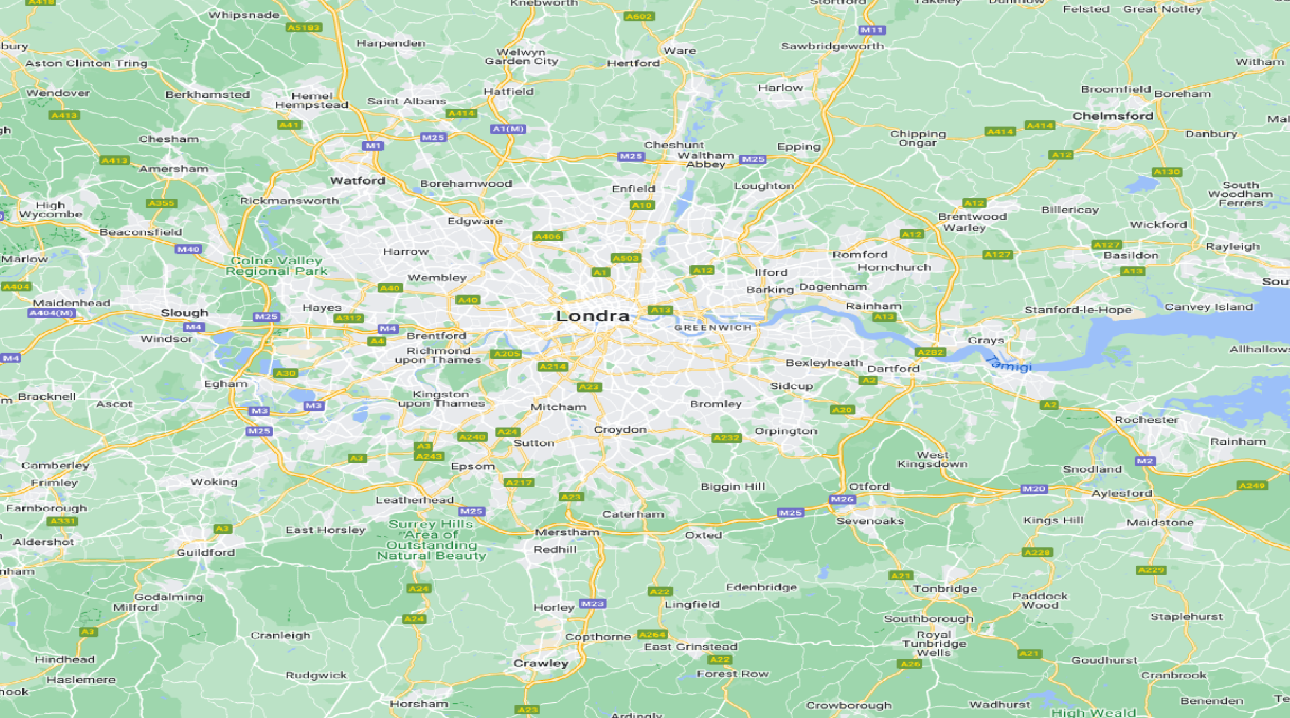
\includegraphics[width=8cm]{images/london_maps.png} }}%
    \subfloat[\centering Night-time lights]{{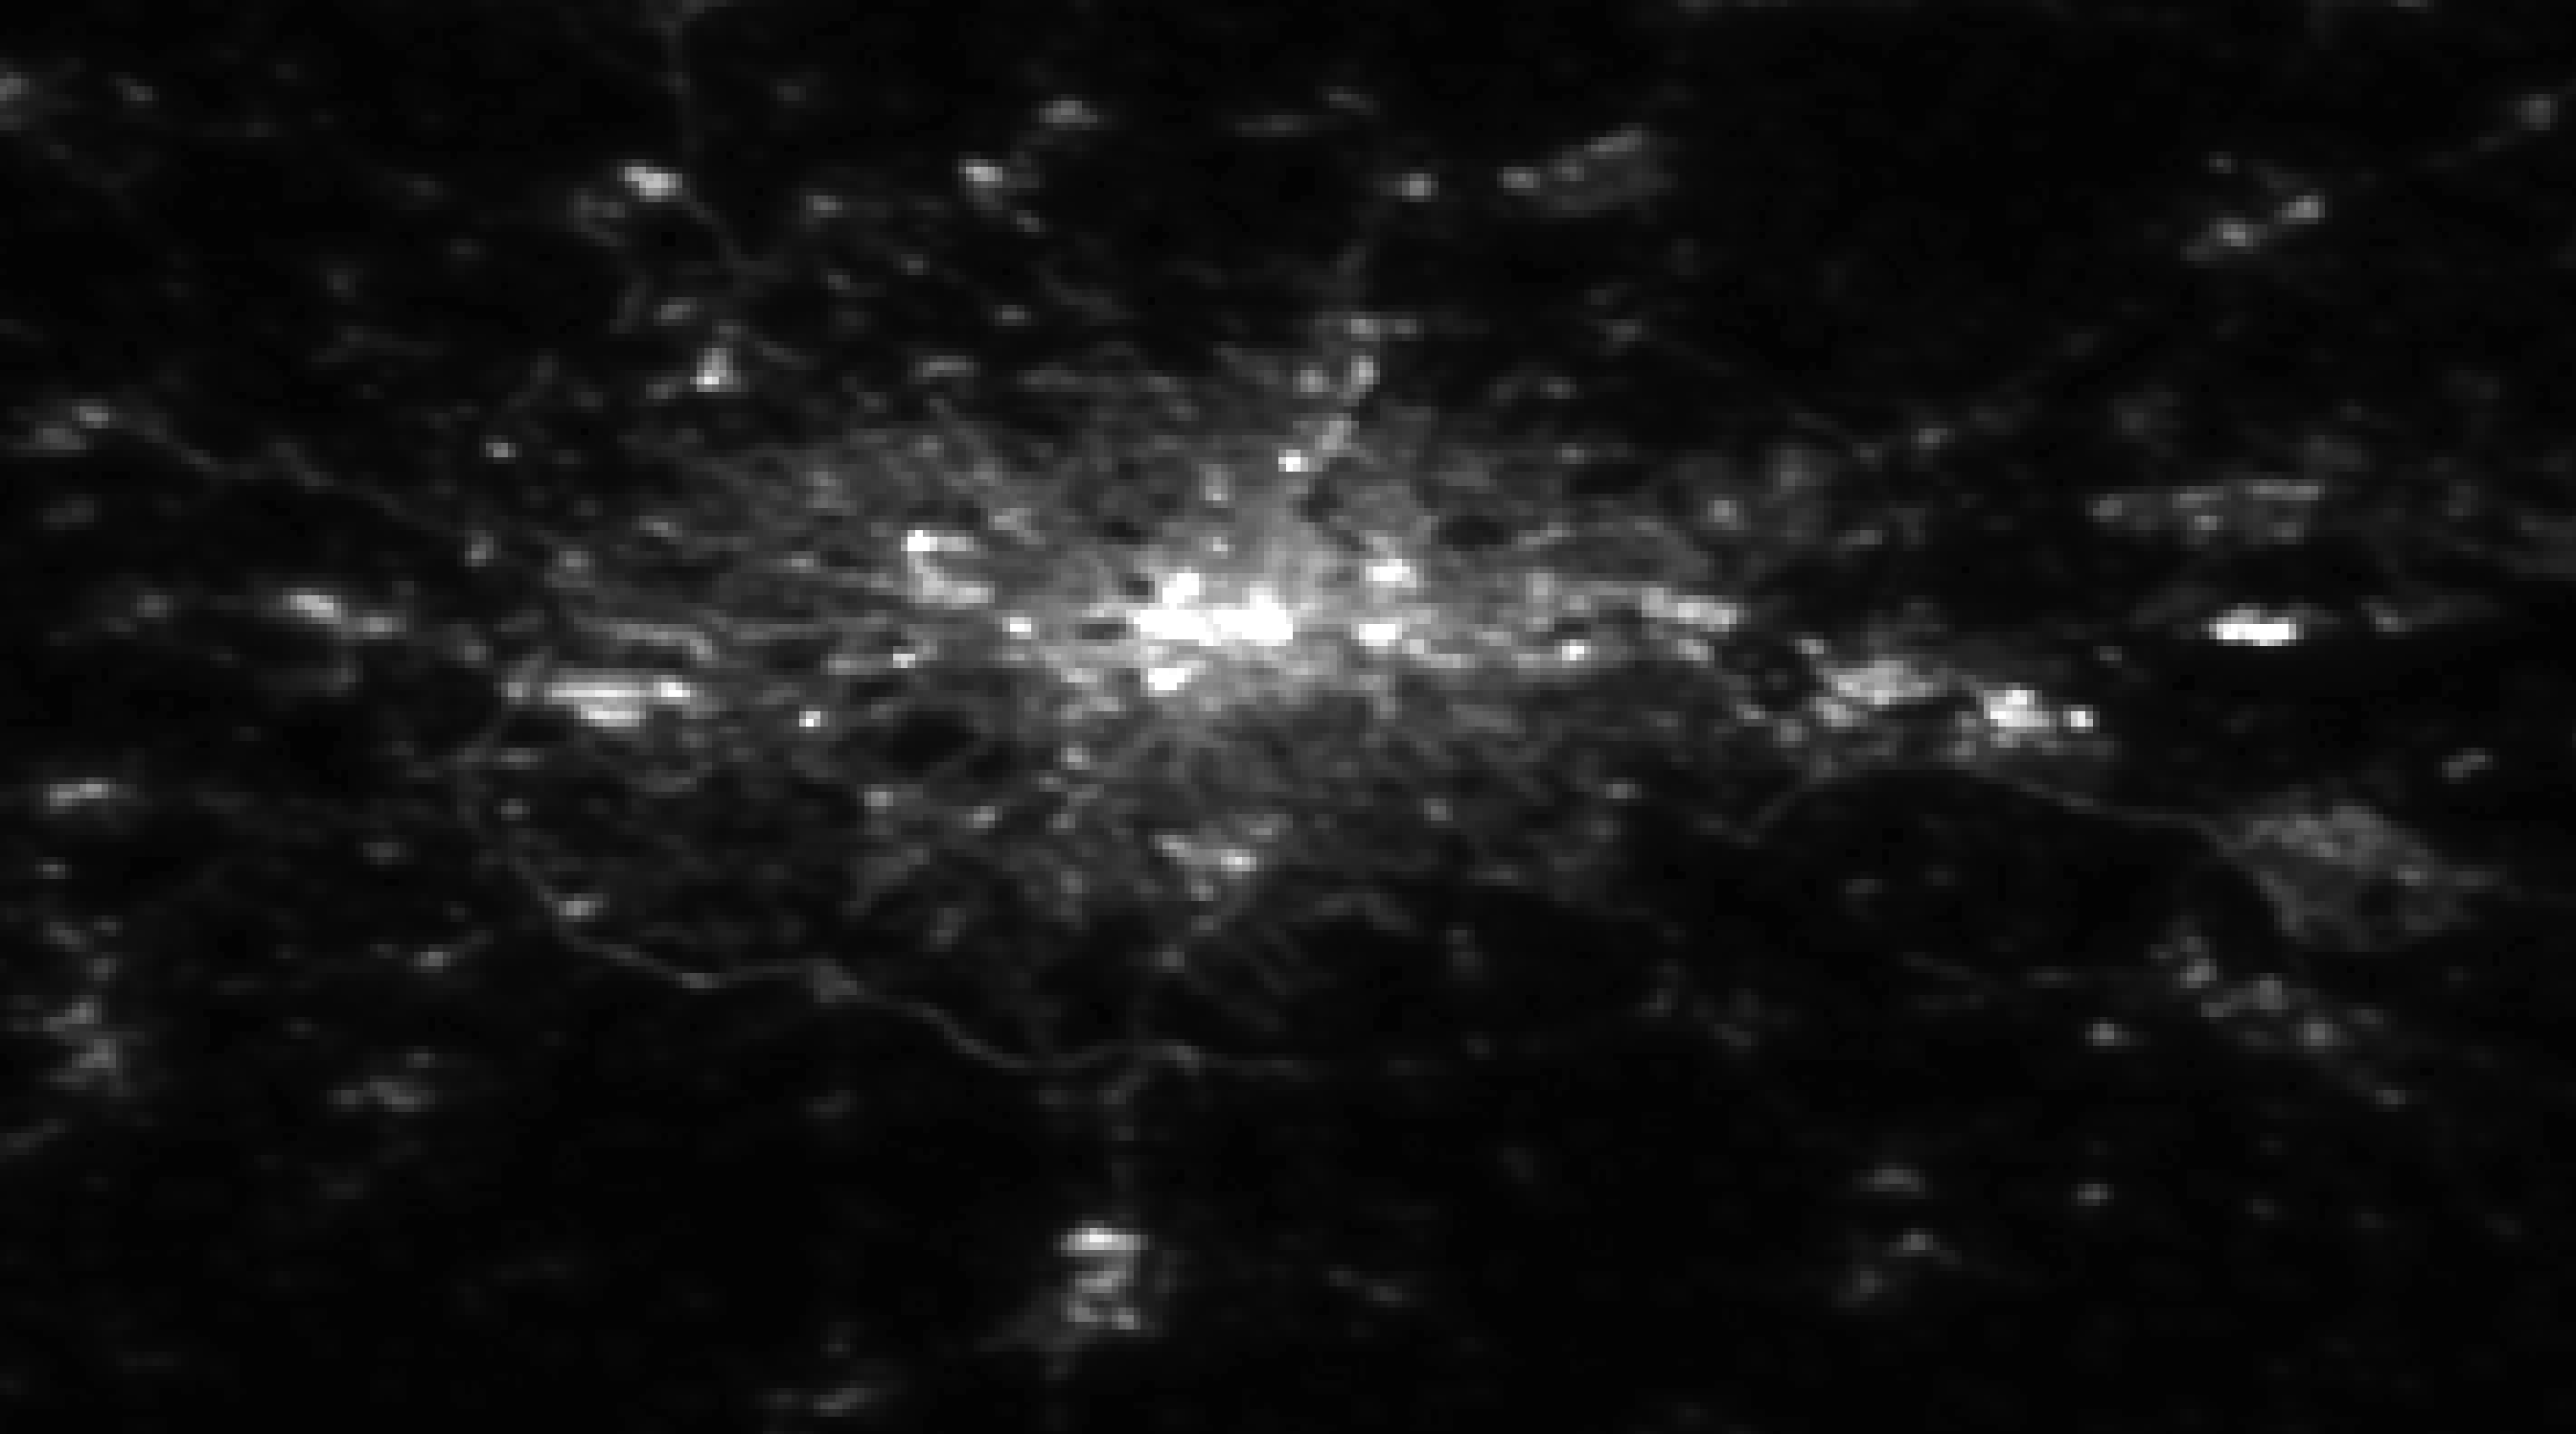
\includegraphics[width=8cm]{images/london_night.png} }}%
    \caption{London - United Kingdom.}%
    \label{fig:london}
\end{figure}

\subsection{Airports}
Airports are usually the brightest part of the cities. In \autoref{fig:malpensa} and in \autoref{fig:charlesdegaulle} two of Europe's busiest airports. The intense night-time lighting is influenced by the traffic and by the dimensions of the airport.
\begin{figure}[h!]
    \hspace*{-2.8cm}
    \centering
    \subfloat[\centering Google Maps]{{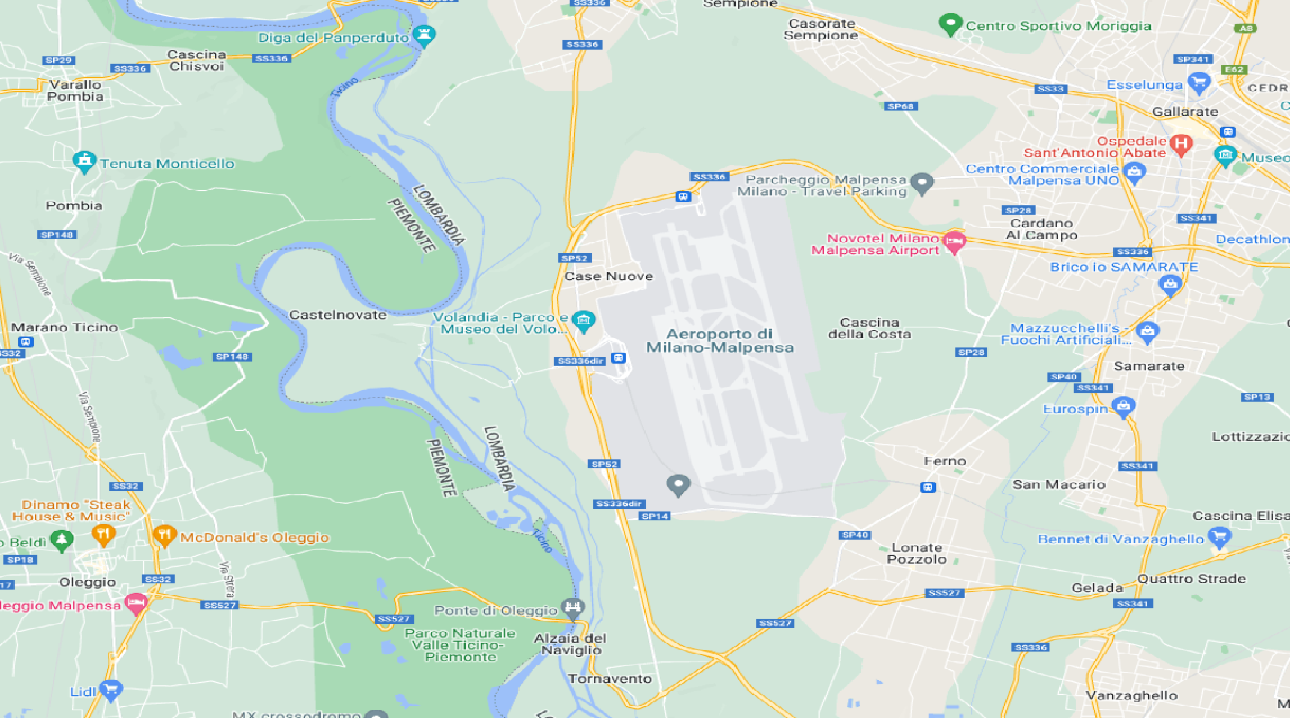
\includegraphics[width=8cm]{images/malpensa_maps.png} }}%
    \subfloat[\centering Night-time lights]{{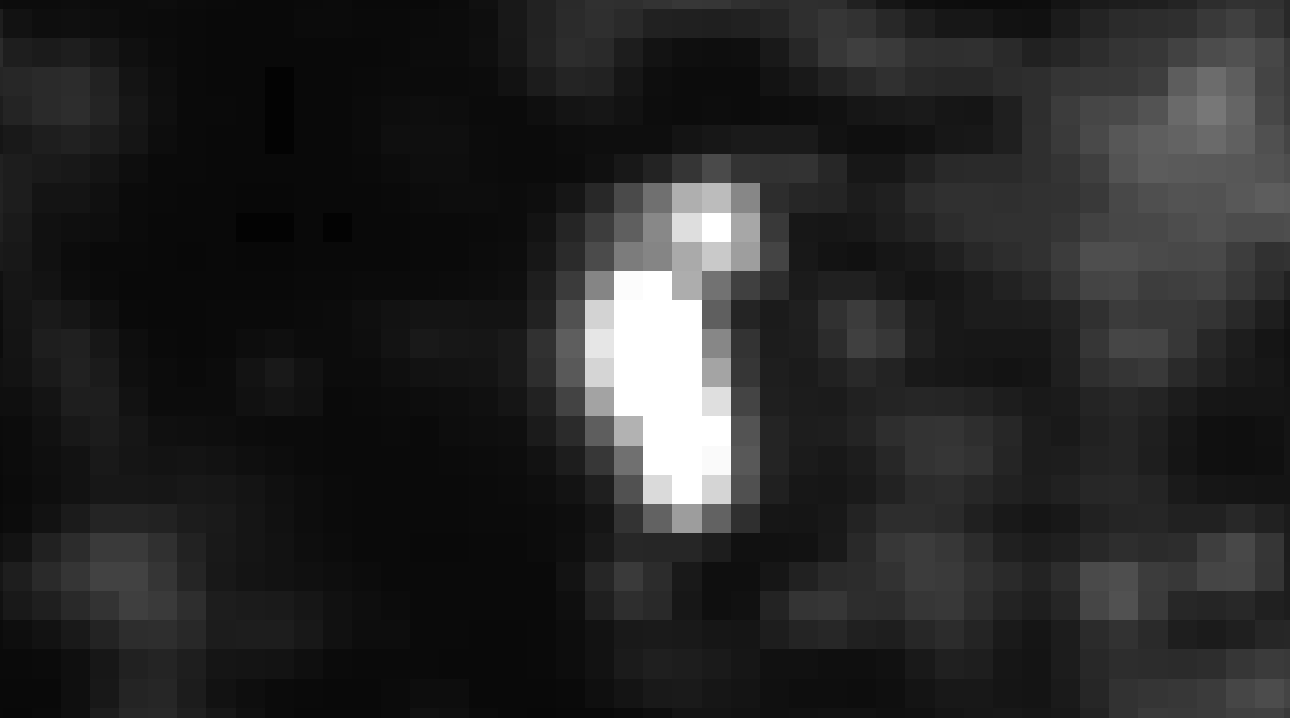
\includegraphics[width=8cm]{images/malpensa_night.png} }}%
    \caption{Malpensa Airport, Milan - Italy.}%
    \label{fig:malpensa}
\end{figure}
\begin{figure}[h!]
    \hspace*{-2.8cm}
    \centering
    \subfloat[\centering Google Maps]{{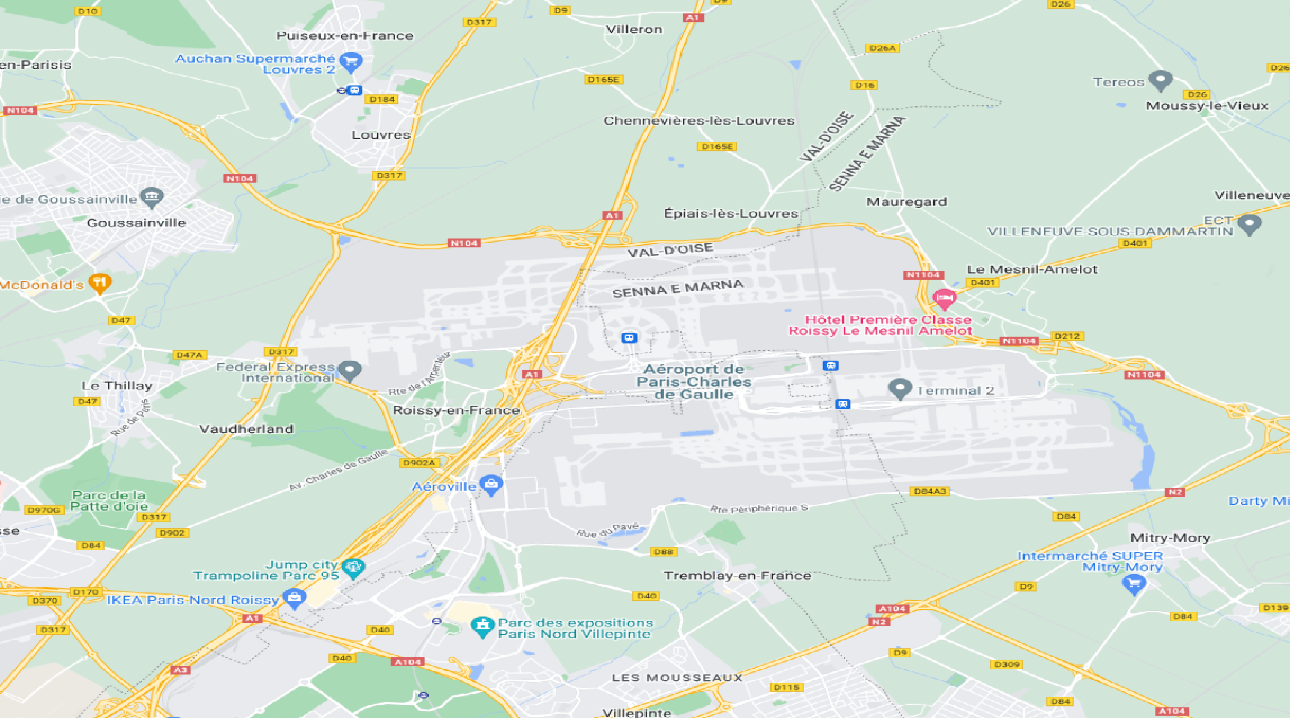
\includegraphics[width=8cm]{images/charlesdegaulle_maps.png} }}%
    \subfloat[\centering Night-time lights]{{
\includegraphics[width=8cm]{images/charlesdegaulle_night.png} }}%
    \caption{Charles De Gaulle Airport, Paris - France.}%
    \label{fig:charlesdegaulle}
\end{figure}
\subsection{Ports}
 In \autoref{fig:rotterdam}, the port of Rotterdam which is one of the largest European commercial ports. The port infrastructure is the main driver of night-time lighting, however docked ships are also a main source.
\begin{figure}[h!]
    \hspace*{-2.8cm}
    \centering
    \subfloat[\centering Google Maps]{{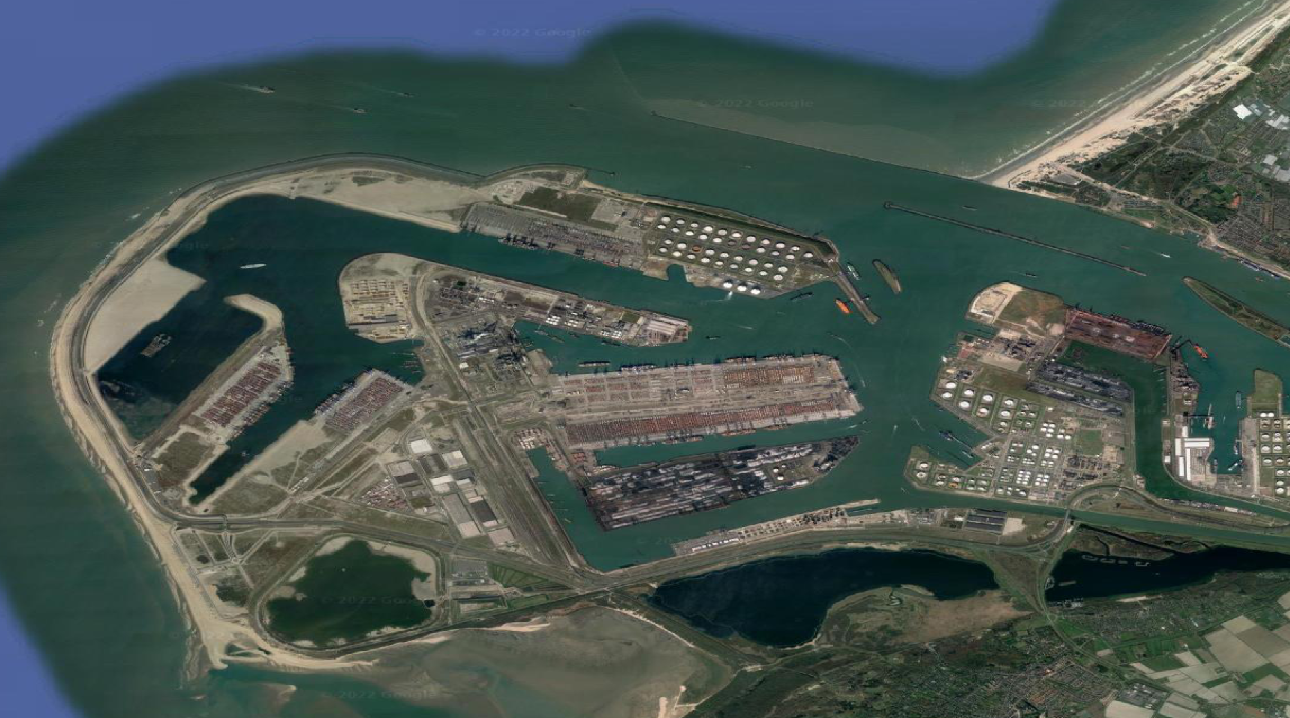
\includegraphics[width=8cm]{images/Rotterdamport_maps.png} }}%
    \subfloat[\centering Night-time lights]{{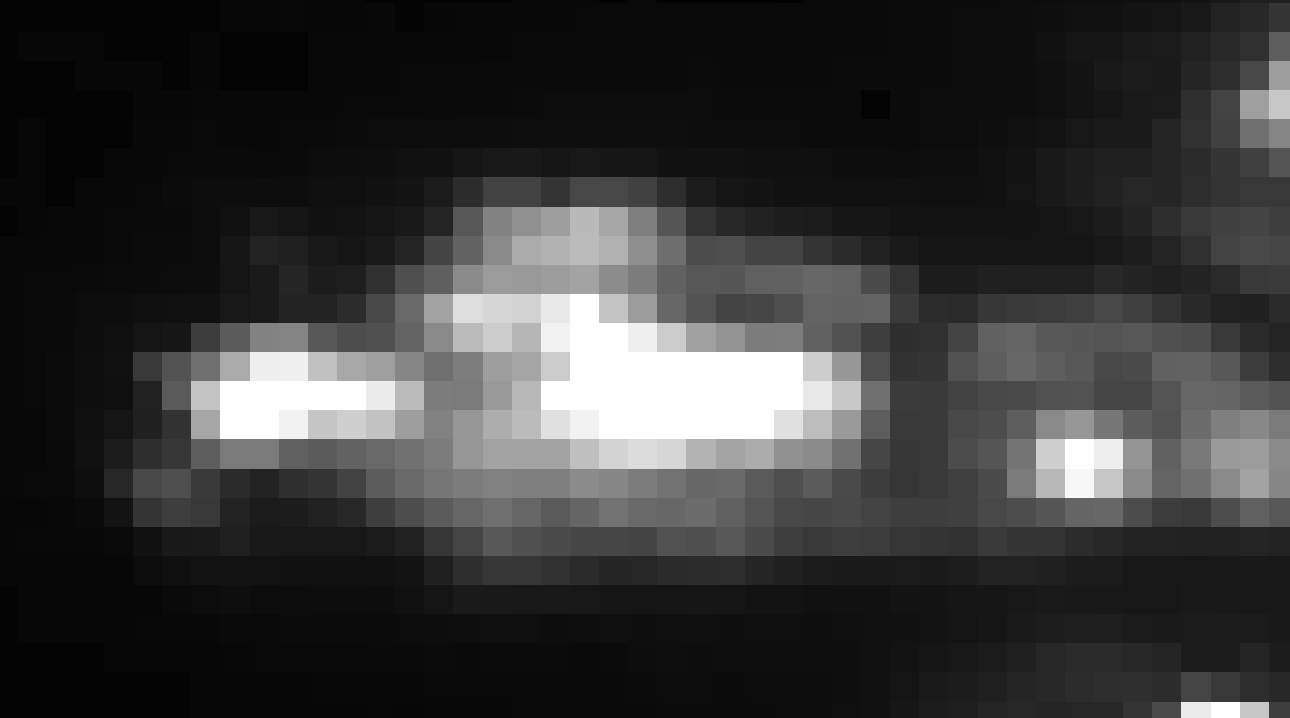
\includegraphics[width=8cm]{images/Rotterdamport_night.png} }}%
    \caption{Rotterdam port - Netherlands.}%
    \label{fig:rotterdam}
\end{figure}
\subsection{Human settlements}
 \autoref{fig:nile} shows the night-time lights image of the Nile river in Egypt. This image is particularly fascinating as it shows a well-known fact in historiography: populations tend to settle around water sources.
 In particular, observing the river delta, it is possible to see how human activities are concentrated, in a web fashion, around its distributaries.
 Indeed, it is unsurprising that most of Egypt's gross domestic product is concentrated around its primary water source.
\begin{figure}[h!]
    \hspace*{-2.8cm}
    \centering
    \subfloat[\centering Google Maps]{{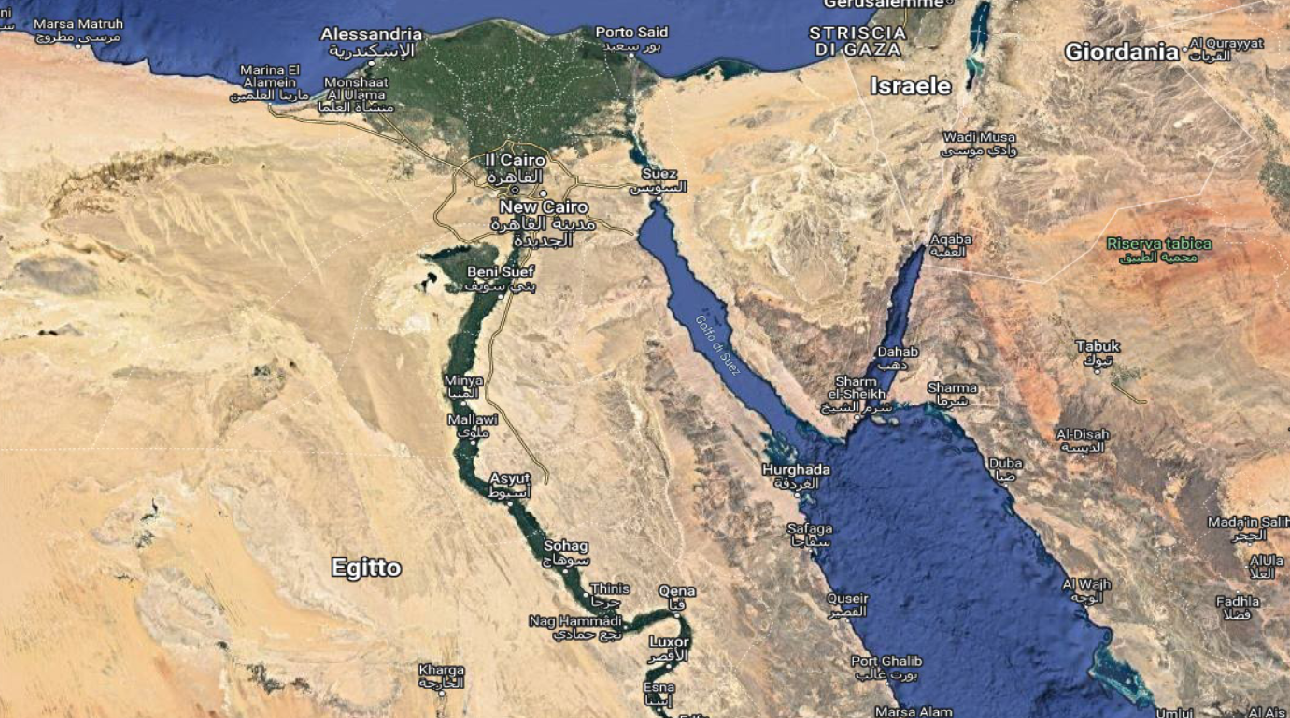
\includegraphics[width=8cm]{images/nile_maps.png} }}%
    \subfloat[\centering Night-time lights]{{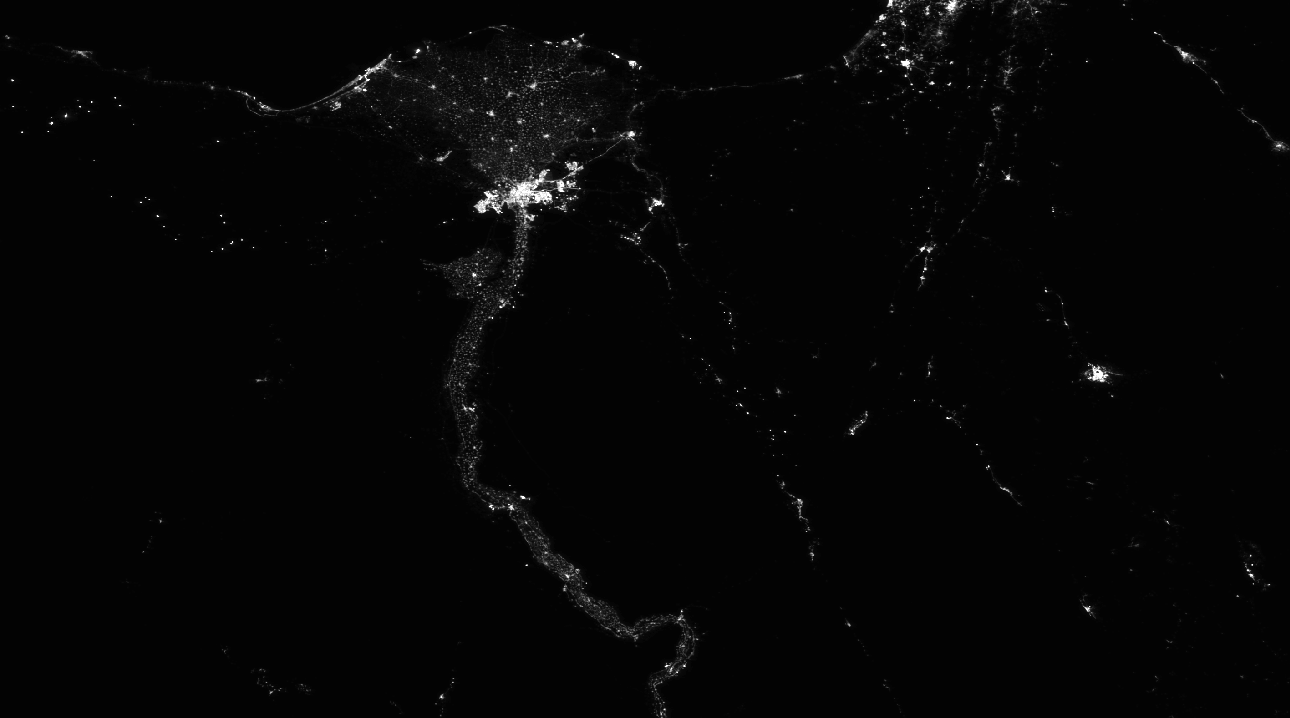
\includegraphics[width=8cm]{images/nile_night.png} }}%
    \caption{Nile river, Egypt.}%
    \label{fig:nile}
\end{figure}

\section{Why night-time lights should be adopted} % \ensuremath{\NoCaseChange{\mathbb{ZNR}}}
The employment of night-time lights makes it possible to estimate economic variables under special conditions in situations where we cannot obtain data or have no guarantee of its truthfulness.
Night-time lights have several interesting properties that have allowed their usage in economic literature. 
\begin{description}
  \item[Exogenous nature:]
 Night-time lights' measurement errors are independent of economic variables' ones \citep{hu2022illuminating}. This is a crucial property, as it will be shown in the next chapters, that allows them to be used as an alternative measure of the economy to improve the estimates of the standard ones. In addition, official growth estimates or forecasts pass through government institutes that may have an interest in manipulating data for their political agenda. Night-time lights observable by satellites are much more challenging to manipulate. 
 
In this regard, a recent working paper \citep{martinez2018much}, forthcoming in the Journal of Political Economy in 2022, shows how autocratic states tend to overstate their growth estimates. Martinez argues that "Since governments themselves usually produce these estimates, they face a recurring temptation to exaggerate just how well the economy is doing".
His results show that the elasticities of night-time lights on GDP are systematically larger in the most authoritarian regimes and that the overestimation averages 35\%.
\item[Worldwide coverage:] night-time lights imagery are captured daily for every area worldwide. This makes it possible to conduct economic estimations in every area of the globe, including countries lacking statistical institutions or areas affected by natural disasters or wars. 

For instance, using data from Project Black Marble, researchers from NASA's Goddard Space Flight Center (GSFC) and the Universities Space Research Association (USRA) analysed the consequences of the Russian invasion of Ukraine on city lights.\footnote{\url{https://earthobservatory.nasa.gov/images/150002/tracking-night-lights-in-ukraine}}
Similarly, \citet{li2018night} studied the dynamics of night-time lights during the Iraqi civil war.
\item[High-frequency data:] data on night-time lights are published daily. As I will show later, for this time span there are substantial data cleaning problems; however, these images lend themselves to daily analysis. Given the long process of estimating official GDP, it can be argued that estimating economic variables through night-time lights leads to high-frequency data. Unfortunately, little has been written about the applicability of economic variables estimated with night-time lights to high-frequency studies. However, also as a result of recent developments in sensor technology (VIIRS), it is possible to consider using these data for policy evaluation analyses.
\item[High-resolution data:]
As I will show in more detail in the following section, the night-time light data is high-resolution data. Namely, we can obtain information for areas of approximately $500mt \times 500mt$.
Using these data to study economic variables allows us to reconstruct economic data and allocate information in space. For instance, it is possible to reconstruct geographic maps by calculating the GDP produced in each square kilometre of a country and thus perform zonal statistics in very small areas. With the high-frequency nature of data, it is possible to monitor a restricted area and observe what happens over time or how the economy of the area evolves following the adoption of a certain policy.
\end{description}
%*****************************************
%*****************************************
%*****************************************
%*****************************************
%*****************************************